%% abtex2-modelo-trabalho-academico.tex, v-1.9.2 laurocesar
%% Copyright 2012-2014 by abnTeX2 group at http://abntex2.googlecode.com/ 
%%
%% This work may be distributed and/or modified under the
%% conditions of the LaTeX Project Public License, either version 1.3
%% of this license or (at your option) any later version.
%% The latest version of this license is in
%%   http://www.latex-project.org/lppl.txt
%% and version 1.3 or later is part of all distributions of LaTeX
%% version 2005/12/01 or later.
%%
%% This work has the LPPL maintenance status `maintained'.
%% 
%% The Current Maintainer of this work is the abnTeX2 team, led
%% by Lauro César Araujo. Further information are available on 
%% http://abntex2.googlecode.com/
%%
%% This work consists of the files abntex2-modelo-trabalho-academico.tex,
%% abntex2-modelo-include-comandos and abntex2-modelo-references.bib
%%

% ------------------------------------------------------------------------
% ------------------------------------------------------------------------
% abnTeX2: Modelo de Trabalho Academico (tese de doutorado, dissertacao de
% mestrado e trabalhos monograficos em geral) em conformidade com 
% ABNT NBR 14724:2011: Informacao e documentacao - Trabalhos academicos -
% Apresentacao
% ------------------------------------------------------------------------
% ------------------------------------------------------------------------

\documentclass[
	% -- opções da classe memoir --
	12pt,               % tamanho da fonte
	openright,          % capítulos começam em pág ímpar (insere página vazia caso preciso)
	twoside,            % para impressão em verso e anverso. Oposto a oneside
	a4paper,            % tamanho do papel. 
	% -- opções da classe abntex2 --
	%chapter=TITLE,     % títulos de capítulos convertidos em letras maiúsculas
	%section=TITLE,     % títulos de seções convertidos em letras maiúsculas
	%subsection=TITLE,  % títulos de subseções convertidos em letras maiúsculas
	%subsubsection=TITLE,% títulos de subsubseções convertidos em letras maiúsculas
	% -- opções do pacote babel --
	english,            % idioma adicional para hifenização
	% french,             % idioma adicional para hifenização
	% spanish,            % idioma adicional para hifenização
	brazil              % o último idioma é o principal do documento
	]{abntex2}

% ---
% Pacotes básicos 
% ---
\usepackage{lmodern}            % Usa a fonte Latin Modern          
\usepackage[T1]{fontenc}        % Selecao de codigos de fonte.
\usepackage[utf8]{inputenc}     % Codificacao do documento (conversão automática dos acentos)
\usepackage{lastpage}           % Usado pela Ficha catalográfica
\usepackage{indentfirst}        % Indenta o primeiro parágrafo de cada seção.
\usepackage{color}              % Controle das cores
\usepackage{graphicx}           % Inclusão de gráficos
\usepackage{microtype}          % para melhorias de justificação
% ---
		
% ---
% Pacotes adicionais, usados apenas no âmbito do Modelo Canônico do abnteX2
% ---
\usepackage{lipsum}             % para geração de dummy text
% ---

% ---
% Pacotes de citações
% ---
\usepackage[brazilian,hyperpageref]{backref}     % Paginas com as citações na bibl
\usepackage[alf]{abntex2cite}   % Citações padrão ABNT

% --- 
% CONFIGURAÇÕES DE PACOTES
% --- 

% ---
% Configurações do pacote backref
% Usado sem a opção hyperpageref de backref
\renewcommand{\backrefpagesname}{Citado na(s) página(s):~}
% Texto padrão antes do número das páginas
\renewcommand{\backref}{}
% Define os textos da citação
\renewcommand*{\backrefalt}[4]{
	\ifcase #1 %
		Nenhuma citação no texto.%
	\or
		Citado na página #2.%
	\else
		Citado #1 vezes nas páginas #2.%
	\fi}%
% ---

% Criando um novo tipo de coluna centralizado e com largura fixa
\newcolumntype{C}[1]{>{\centering\let\newline\\\arraybackslash\hspace{0pt}}m{#1}}


% ---
% Informações de dados para CAPA e FOLHA DE ROSTO
% ---
\titulo{Análise Comparativa de Técnicas de Extração de Metadados em Artigos Científicos sob o Ponto de Vista do Resultado Comparativo Final}
\autor{José Alberto Grossi Júnior}
\local{Belo Horizonte/MG, Brasil}
\data{2014, v-0.1.1}
\orientador{Marcello Peixoto Bax}
\instituicao{%
	Universidade Federal de Minas Gerais -- UFMG
	\par
	Escola de Ciência da Informação
	\par
	Programa de Pós-Graduação em Ciência da Informação}
\tipotrabalho{Dissertação (Mestrado)}
% O preambulo deve conter o tipo do trabalho, o objetivo, 
% o nome da instituição e a área de concentração 
\preambulo{Dissertação de mestrado apresentada à coordenação do PPGCI/UFMG com o objetivo de obtenção de título de Mestre em Ciência da Informação}
% ---


% ---
% Configurações de aparência do PDF final

% alterando o aspecto da cor azul
\definecolor{blue}{RGB}{41,5,195}

% informações do PDF
\makeatletter
\hypersetup{
		%pagebackref=true,
		pdftitle={\@title}, 
		pdfauthor={\@author},
		pdfsubject={\imprimirpreambulo},
		pdfcreator={LaTeX with abnTeX2},
		pdfkeywords={extracao}{metadados}{artigos cientificos}{tecnicas de extracao}, 
		colorlinks=true,            % false: boxed links; true: colored links
		linkcolor=blue,             % color of internal links
		citecolor=blue,             % color of links to bibliography
		filecolor=magenta,              % color of file links
		urlcolor=blue,
		bookmarksdepth=4
}
\makeatother
% --- 

% --- 
% Espaçamentos entre linhas e parágrafos 
% --- 

% O tamanho do parágrafo é dado por:
\setlength{\parindent}{1.3cm}

% Controle do espaçamento entre um parágrafo e outro:
\setlength{\parskip}{0.2cm}  % tente também \onelineskip

% ---
% compila o indice
% ---
\makeindex
% ---

% ----
% Início do documento
% ----
\begin{document}

% Retira espaço extra obsoleto entre as frases.
\frenchspacing 

% ----------------------------------------------------------
% ELEMENTOS PRÉ-TEXTUAIS
% ----------------------------------------------------------
% \pretextual

% ---
% Capa
% ---
\imprimircapa
% ---

% ---
% Folha de rosto
% (o * indica que haverá a ficha bibliográfica)
% ---
\imprimirfolhaderosto*
% ---

% ---
% Inserir a ficha bibliografica
% ---

% Isto é um exemplo de Ficha Catalográfica, ou ``Dados internacionais de
% catalogação-na-publicação''. Você pode utilizar este modelo como referência. 
% Porém, provavelmente a biblioteca da sua universidade lhe fornecerá um PDF
% com a ficha catalográfica definitiva após a defesa do trabalho. Quando estiver
% com o documento, salve-o como PDF no diretório do seu projeto e substitua todo
% o conteúdo de implementação deste arquivo pelo comando abaixo:
%
% \begin{fichacatalografica}
%     \includepdf{fig_ficha_catalografica.pdf}
% \end{fichacatalografica}
\begin{fichacatalografica}
	\vspace*{\fill}                 % Posição vertical
	\hrule                          % Linha horizontal
	\begin{center}                  % Minipage Centralizado
	\begin{minipage}[c]{12.5cm}     % Largura
	
	\imprimirautor
	
	\hspace{0.5cm} \imprimirtitulo  / \imprimirautor. --
	\imprimirlocal, \imprimirdata-
	
	\hspace{0.5cm} \pageref{LastPage} p. : il. (algumas color.) ; 30 cm.\\
	
	\hspace{0.5cm} \imprimirorientadorRotulo~\imprimirorientador\\
	
	\hspace{0.5cm}
	\parbox[t]{\textwidth}{\imprimirtipotrabalho~--~\imprimirinstituicao,
	\imprimirdata.}\\
	
	\hspace{0.5cm}
		1. Extração de informação
		2. Metadados.
		I. Artigos científicos.
		II. Universidade Federal de Minas Gerais.
		III. Escola de Ciência da Informação.
		IV. \imprimirtitulo\\            
	
	\hspace{8.75cm} CDU 02:141:005.7\\
	
	\end{minipage}
	\end{center}
	\hrule
\end{fichacatalografica}
% ---

% % ---
% % Inserir errata
% % ---
% \begin{errata}
% Elemento opcional da \citeonline[4.2.1.2]{NBR14724:2011}. Exemplo:

% \vspace{\onelineskip}

% FERRIGNO, C. R. A. \textbf{Tratamento de neoplasias ósseas apendiculares com
% reimplantação de enxerto ósseo autólogo autoclavado associado ao plasma
% rico em plaquetas}: estudo crítico na cirurgia de preservação de membro em
% cães. 2011. 128 f. Tese (Livre-Docência) - Faculdade de Medicina Veterinária e
% Zootecnia, Universidade de São Paulo, São Paulo, 2011.

% \begin{table}[htb]
% \center
% \footnotesize
% \begin{tabular}{|p{1.4cm}|p{1cm}|p{3cm}|p{3cm}|}
%   \hline
%    \textbf{Folha} & \textbf{Linha}  & \textbf{Onde se lê}  & \textbf{Leia-se}  \\
% 	\hline
% 	1 & 10 & auto-conclavo & autoconclavo\\
%    \hline
% \end{tabular}
% \end{table}

% \end{errata}
% ---

% ---
% Inserir folha de aprovação
% ---

% Isto é um exemplo de Folha de aprovação, elemento obrigatório da NBR
% 14724/2011 (seção 4.2.1.3). Você pode utilizar este modelo até a aprovação
% do trabalho. Após isso, substitua todo o conteúdo deste arquivo por uma
% imagem da página assinada pela banca com o comando abaixo:
%
% \includepdf{folhadeaprovacao_final.pdf}
%
\begin{folhadeaprovacao}

  \begin{center}
	{\ABNTEXchapterfont\large\imprimirautor}

	\vspace*{\fill}\vspace*{\fill}
	\begin{center}
	  \ABNTEXchapterfont\bfseries\Large\imprimirtitulo
	\end{center}
	\vspace*{\fill}
	
	\hspace{.45\textwidth}
	\begin{minipage}{.5\textwidth}
		\imprimirpreambulo
	\end{minipage}%
	\vspace*{\fill}
   \end{center}
		
   Trabalho aprovado. \imprimirlocal, 20 de setembro de 2014:

   \assinatura{\textbf{\imprimirorientador} \\ Orientador} 
   \assinatura{\textbf{Professor} \\ Professor Convidado 1}
   \assinatura{\textbf{Professor} \\ Professor Convidado 2}
   \assinatura{\textbf{Professor} \\ Professor Convidado 3}
   %\assinatura{\textbf{Professor} \\ Convidado 4}
	  
   \begin{center}
	\vspace*{0.5cm}
	{\large\imprimirlocal}
	\par
	{\large\imprimirdata}
	\vspace*{1cm}
  \end{center}
  
\end{folhadeaprovacao}
% ---

% ---
% Dedicatória
% ---
\begin{dedicatoria}
   \vspace*{\fill}
   \centering
   \noindent
   \textit{ Este trabalho é dedicado a todas as pessoas que desejam,\\ 
   de uma forma ou outra, superar seus objetivos pessoais.} \vspace*{\fill}
\end{dedicatoria}
% ---

% ---
% Agradecimentos
% ---
\begin{agradecimentos}
A escrever.
% Os agradecimentos principais são direcionados à Gerald Weber, Miguel Frasson,
% Leslie H. Watter, Bruno Parente Lima, Flávio de Vasconcellos Corrêa, Otavio Real
% Salvador, Renato Machnievscz\footnote{Os nomes dos integrantes do primeiro
% projeto abn\TeX\ foram extraídos de
% \url{http://codigolivre.org.br/projects/abntex/}} e todos aqueles que
% contribuíram para que a produção de trabalhos acadêmicos conforme
% as normas ABNT com \LaTeX\ fosse possível.

% Agradecimentos especiais são direcionados ao Centro de Pesquisa em Arquitetura
% da Informação\footnote{\url{http://www.cpai.unb.br/}} da Universidade de
% Brasília (CPAI), ao grupo de usuários
% \emph{latex-br}\footnote{\url{http://groups.google.com/group/latex-br}} e aos
% novos voluntários do grupo
% \emph{\abnTeX}\footnote{\url{http://groups.google.com/group/abntex2} e
% \url{http://abntex2.googlecode.com/}}~que contribuíram e que ainda
% contribuirão para a evolução do \abnTeX.

\end{agradecimentos}
% ---

% ---
% Epígrafe
% ---
% \begin{epigrafe}
% 	\vspace*{\fill}
% 	\begin{flushright}
% 		\textit{``Não vos amoldeis às estruturas deste mundo, \\
% 		mas transformai-vos pela renovação da mente, \\
% 		a fim de distinguir qual é a vontade de Deus: \\
% 		o que é bom, o que Lhe é agradável, o que é perfeito.\\
% 		(Bíblia Sagrada, Romanos 12, 2)}
% 	\end{flushright}
% \end{epigrafe}
% ---

% ---
% RESUMOS
% ---

% resumo em português
\setlength{\absparsep}{18pt} % ajusta o espaçamento dos parágrafos do resumo
\begin{resumo}
 % Segundo a \citeonline[3.1-3.2]{NBR6028:2003}, o resumo deve ressaltar o
 % objetivo, o método, os resultados e as conclusões do documento. A ordem e a extensão
 % destes itens dependem do tipo de resumo (informativo ou indicativo) e do
 % tratamento que cada item recebe no documento original. O resumo deve ser
 % precedido da referência do documento, com exceção do resumo inserido no
 % próprio documento. (\ldots) As palavras-chave devem figurar logo abaixo do
 % resumo, antecedidas da expressão Palavras-chave:, separadas entre si por
 % ponto e finalizadas também por ponto.

 % \textbf{Palavras-chaves}: latex. abntex. editoração de texto.

    A necessidade de contribuição entre a comunidade acadêmica é evidente quando da necessidade de leituras específicas de artigos científicos de autores espalhados pelo mundo. Porém, esta contribuição se dá de maneira muito pessoal, com envios manuais de artigos quando da necessidade de certos nichos acadêmicos. A dificuldade apresentada geralmente é a centralização de artigos de maneira livre e compensatória, por meio de extração automática de metadados relevantes para o catálogo destes documentos, de maneira a permitir que qualquer pesquisador, devidamente reconhecido, possa compartilhar e obter estes documentos de maneira eficaz e anônima.

    Este trabalho demonstra que as técnicas livres existentes para extração de metadados em artigos científicos não são suficientes para abranger os diversos formatos existentes de apresentação dos conteúdos, uma vez que são baseados em layout pré-definidos, sem possibilidade de expansão ou adaptação de acordo com a necessidade de certos grupos de pesquisa, cujo formato de apresentação deste tipo de documento se dá de maneira diferenciada, ou até mesmo, adaptada para seu universo de pesquisadores.

    \textbf{Palavras-chaves}: artigos científicos. extração de metadados. extração de dados em artigos.


\end{resumo}

% resumo em inglês
\begin{resumo}[Abstract]
 \begin{otherlanguage*}{english}
	
	The need of contribution existent in the academic community is focused based on the sharing of papers from authors around the world, when specific studies are needed. However, this contribution is made in a very basic and personal way, with papers sent by manual interactions from some specific research groups. The main goal is focused on the papers centralization in a free and compensatory format, by automatic relevant metadata extraction to the indexation of these documents, allowing any researcher to share and get these documents in a very effective manner. 

	This work shows how the existent metadata extraction techniques in scientific papers are not totally perfect to perform the different papers formats to present research works, once they are based on pre-defined layouts, without any change of customization according with some groups needs, because of a different presentation format, or even, adapted to your researchers' worlds.

    \textbf{Palavras-chaves}: scientific papers. metadata extraction. data extraction on scientific papers.

   % \vspace{\onelineskip}
 
   % \noindent 
   % \textbf{Key-words}: latex. abntex. text editoration.
 \end{otherlanguage*}
\end{resumo}

% resumo em francês 
% \begin{resumo}[Résumé]
%  \begin{otherlanguage*}{french}
% 	Il s'agit d'un résumé en français.
 
%    \textbf{Mots-clés}: latex. abntex. publication de textes.
%  \end{otherlanguage*}
% \end{resumo}

% % resumo em espanhol
% \begin{resumo}[Resumen]
%  \begin{otherlanguage*}{spanish}
%    Este es el resumen en español.
  
%    \textbf{Palabras clave}: latex. abntex. publicación de textos.
%  \end{otherlanguage*}
% \end{resumo}
% ---

% ---
% inserir lista de ilustrações
% ---
\pdfbookmark[0]{\listfigurename}{lof}
\listoffigures*
\cleardoublepage
% ---

% ---
% inserir lista de tabelas
% ---
\pdfbookmark[0]{\listtablename}{lot}
\listoftables*
\cleardoublepage
% ---

% ---
% inserir lista de abreviaturas e siglas
% ---
\begin{siglas}
  \item[PDF] Portable Document Format
  \item[IEEE] Institute of Electrical and Electronics Engineers
  \item[RSL] Revisão Sistemática de Literatura
  \item[ACM] Association for Computing Machinery
  \item[CAPES] Coordenação de Aperfeiçoamento de Pessoal de Nível Superior
  \item[XML] eXtensible Markup Language
  \item[SVM] Support Vector Machines
  \item[HMM] Hidden Markov Models
  \item[CRF] Conditional Random Fields
\end{siglas}
% ---

% ---
% inserir lista de símbolos
% ---
% \begin{simbolos}
  % \item[$ \Gamma $] Letra grega Gama
  % \item[$ \Lambda $] Lambda
  % \item[$ \zeta $] Letra grega minúscula zeta
  % \item[$ \in $] Pertence
% \end{simbolos}
% ---

% ---
% inserir o sumario
% ---
\pdfbookmark[0]{\contentsname}{toc}
\tableofcontents*
\cleardoublepage
% ---



% ----------------------------------------------------------
% ELEMENTOS TEXTUAIS
% ----------------------------------------------------------
\textual

% ----------------------------------------------------------
% Introdução (exemplo de capítulo sem numeração, mas presente no Sumário)
% ----------------------------------------------------------
\chapter[Introdução]{Introdução}
% \addcontentsline{toc}{chapter}{Introdução}
% ----------------------------------------------------------

A necessidade de contribuição acontece de forma natural no ser humano. Os desejos em ajudar ao próximo e inclusive contribuir com alguma parte de sua formação é algo que desperta um desejo cada vez mais amplo do ponto de vista social.

Somos seres realizados pela satisfação do outro, e seu sucesso de uma forma ou outra acarreta em nosso sucesso, nossa satisfação pessoal e de certa forma profissional. Sentimos atraídos por contribuir e por compartilhar conhecimento, sendo ele umas das principais formas de realização como pessoa.

Com o crescimento da pesquisa em todo o mundo um grande número de publicações foram inseridas no meio, fazendo com que uma infinidade de material esteja disponível em poucos segundos. Deste modo, a necessidade de centralização automatizada dos dados e a contribuição dentre os pesquisadores é inerente ao desenvolvimento desta área. 

No âmbito acadêmico sempre contribuímos de uma forma ou outra com a formação de nossos colegas e parceiros de pesquisa. Esta contribuição pode ser feita com base em uma conversa informal ou até mesmo com uma ajuda em documentação ou sugestão de um texto para leitura. Esta sugestão de leitura geralmente possui um caráter muito técnico, e envolve na maioria dos casos a utilização de artigos acadêmicos.

Sabemos da existência de bases de conhecimento de maneira global e nacional, porém quando estamos falando da contribuição social, em pequena escala, interpessoal, estamos falando que contribuições físicas, com envio de sugestões de artigos para nossos amigos pesquisadores. Este envio é feito de maneira informal, e reduz tempo e aumenta consequentemente a praticidade do processo de pesquisa.

Sendo assim, esta experiência como objetivo global seria uma ferramenta poderosa de apoio à pesquisa, com pesquisadores compartilhando conhecimentos de maneira informal, anônima, e segura. Esta forma de disseminação de conhecimento traria um benefício muito grande socialmente falando, uma vez que pesquisadores iriam se unir, mesmo que virtualmente, na transmissão de conhecimento entre si próprios, fazendo do processo de pesquisa um processo mais focado e evitando o desperdício de tempo durante a fase de pesquisa e busca por conhecimento.

Para isso, a utilização de técnicas de extração de metadados deve ser utilizada de maneira eficaz, para que de maneira automática diversos artigos sejam analisados e catalogados em pequenos universos de pesquisa. Entende-se por metadados os campos básicos e necessários para que uma pesquisa por nome, por exemplo, seja feita com sucesso. Resume-se então que os metadados que esperam-se ser extraídos destes artigos são: o título do artigo, o nome e e-mail de seus autores, o resumo/abstract e as referências utilizadas.

Basicamente estes campos já permitem que uma pesquisa mais detalhada fosse feita e então o artigo localizado. Já as referências são necessárias para se fazer referências inversas de autores que publicam e são citados posteriormente, facilitando ainda mais aos pesquisadores poder, por exemplo, encontrar artigos semelhantes de uma mesma área do conhecimento.

\begin{figure}
\centering
\caption{Processo de Extração de Metadados}
\label{fig:introducao}
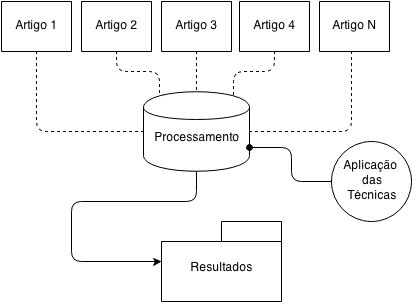
\includegraphics[width=0.7\linewidth]{./assets/introducao}
\end{figure}


\section{Delimitação do Problema}

De modo geral, as técnicas livre existentes para que essa extração de metadados seja feita são focadas em layouts pré-definidos, geralmente de conferências e/ou congressos internacionais, que possuem um padrão visual parecido, como é o caso do IEEE por exemplo, que segue de referência para diversos outros eventos tomando seu layout como base.

Porém, existem diversos outros eventos que possuem layouts de artigos considerados fora do padrão e, portanto, necessitam de adaptações destas técnicas para que seus trabalhos possam ser analisados e catalogados de maneira eficaz. Esta customização promoveria uma série de tentativas para verificar o melhor layout para ser utilizado em cada caso, automaticamente.

\section{Objetivo Geral}

Este trabalho possui como objetivo geral provar que as técnicas livres de extração automática de metadados em artigos científicos ainda necessitam ajustes e principalmente flexibilidade para abranger um maior números de documentos e prover então uma contribuição maior perante a comunidade acadêmica.

A necessidade de customização é uma tendência natural de qualquer ramo de atividade, de maneira a promover possibilidades de ferramentas auto-suficientes capazes de suprir as necessidades de grupos específicos de pesquisas, de eventos ou conferências, que possui padrões de apresentação de artigos personalizados e que demandam de uma análise diferenciada para que possa ser indexada e então analisada por sistemas de informação.

\subsection{Objetivos Específicos}

Com base na diferenciação de formas de apresentação de artigos científicos este trabalho tem como Objetivos Específicos identificar pontos em que técnicas de extração de metadados necessitam de adaptações flexíveis por parte da comunidade em geral, permitindo que artigos sejam analisados de maneira diferente em virtude de especificações distintas e necessidades diferenciadas de grupos de pesquisa.

Os padrões existentes no mercado são de maneira geral insuficientes para suprir as necessidades dos mais diversos eventos e/ou conferências existentes, afunilando a apenas uma pequena parcela de artigos, o que acaba gerando um desconforto e uma ineficácia das técnicas de extração de metadados existentes atualmente.

\section{Resultados Esperados}

As formas de extração de dados em artigos científicos são geralmente baseadas em layouts, ou seja, em pequenos pedaços onde certas informações devem ser informadas. Porém em virtude da grande diversidade de materiais produzidos e em função das adaptações realizadas por grupos e/ou eventos de pesquisa, este layout padrão não se mostra eficiente na abrangência total das necessidades do meio. 

Assim sendo, espera-se que certos artigos científicos não tenham seus metadados analisados de maneira eficaz por todas as técnicas livres existentes de extração de dados, uma vez que adaptações são necessárias a fim de contribuir para uma globalização destas análises, permitindo a customização então de técnicas de extração com base em mercados ou culturas diferentes.

\section{Limitações do Trabalho}

Este trabalho limita-se aos artigos científicos difundidos na comunidade científica em formato PDF, excluindo aqueles em que seu conteúdo é disponibilizados através de imagens escaneadas de documentos físicos, o que impede, em um primeiro momento, de ter os textos analisados em sua forma original, sem necessidade de processamento extra a fim de obter todo o material textual contido em tais imagens.

Além disso o trabalho pressupõe que a língua inglesa seja utilizada como padrão no meio, de maneira a permitir que através de um único idioma o conhecimento seja difundido e aplicado em diversas culturas, independente de especificidades e diferenças culturais, permitindo uma difusão do conhecimento em sua mais pura forma de apresentação.

% Sobre os servidores com Windows

Já na questão de testes de cada técnica de extração de metadados, as técnicas que serão selecionadas deverão ser livres, ou seja, ter seu uso liberado sem a necessidade de pagamento de licenças. Deste modo excluímos todas as técnicas que rodam exclusivamente em plataforma Windows, por exigir licenças de software e fugirem das previsões de teste deste projeto. Assim, os projetos deverão necessariamente utilizar de linguagens de programação livres (ou de código aberto) e que rodem em sistemas operacionais derivados do Unix, como o Linux, por exemplo.

\section{Justificativa}

De maneira geral, a necessidade de centralizar estes artigos científicos existe, e a contribuição seria uma forma de aumentar cada vez mais o acesso aos materiais de pesquisa. Sendo assim, esta forma de análise e extração de metadados traria benefícios para que este repositório fosse criado, tendo então milhões e milhões de documentos em suas bases de dados.

Este trabalho é feito justamente para prover esta visão do que ainda precisa ser melhorado e pensado para que estas técnicas abranjam diversos padrões encontrados no mercado, permitindo além que usuários possam contribuir com seus próprios padrões.

\section{Estrutura}

Esta pesquisa é estruturada iniciando com uma introdução sobre o tema, a definição do problema, os objetivos gerais e específicos e sua justificativa.

O segundo capítulo tem como base o referencial teórico feito através de uma RSL (Revisão Sistemática de Literatura), tendo como base \cite{rsl-manual}, que propõe um passo-a-passo para um revisão de literatura eficaz e atingindo os resultados desejáveis pela pesquisa.

No terceiro capítulo temos a metodologia para o desenvolvimento do trabalho, as técnicas que serão aplicadas e principalmente como serão feitas. Posteriormente, no capítulo quarto temos os testes propriamente ditos, como eles foram realizados, os ambientes de teste, a seleção de artigos para testes e no quinto capítulo os resultados obtidos.

No sexto capítulo temos a conclusão, trabalhos futuros e considerações finais sobre o trabalho apresentado.

\chapter{Revisão de Literatura}

% Falar sobre RSL

Visando obter uma revisão de literatura eficaz foi feita uma Revisão Sistemática de Literatura, com base no Relatório Técnico de \cite{rsl-manual}. Desde modo o projeto se torna mas abrangente do ponto de vista de pesquisa literária e ao mesmo tempo mais restritivo, realmente realizando o estudo dos objetos que são importantes para a pesquisa em si.

% Bases pesquisadas

Basicamente, como o objetivo do trabalho tem foco na resultado prático, geralmente as bases relacionadas às áreas mais técnicas, como Ciência da Computação, devem ser bem focadas, como IEEE e ACM, por exemplo. Outras bases de natureza mais genérica também foram pesquisadas, geralmente através do site da CAPES, mas com caráter mais de apoio teórico realmente.

Embora a amplitude desta área, alguns detalhes necessitam ser observados para evitar assim redundância e perda de foco no trabalho. Basicamente a pesquisa necessitava ser focada em técnicas de extração de dados em artigos científicos, somente. Estas técnicas necessitam ser reais, de maneira a existir realmente uma forma prática de serem testadas, fazendo assim com que os resultados obtidos sejam comparados e confrontados para verificar então a eficácia do processo.

Como a pesquisa necessita de um resultado prático eficaz os critérios que serão adotados para demonstrar a relevância de um estudo serão seus resultados. Com base em uma técnica potencialmente eficaz, sua implantação deve ser realizada, independente da linguagem de programação, e então testada juntamente com um grupo de artigos previamente selecionados como teste base. Estes artigos já possuirão seus dados mapeados de maneira a poder comparar os resultados obtidos com cada uma das técnicas e os resultados então esperados. Portanto os critérios utilizados serão de natureza explicitamente prática, com foco em resultados concretos.

% Falar sobre os eventos encontrados na área

Seguindo as orientações propostas em \cite{rsl-manual} foram mapeados alguns eventos para serem pesquisados, a fim de encontrar trabalhos relevantes para a área. Sendo assim, foram mapeados os seguintes eventos:

\begin{itemize}
\item KDIR (International Conference of Knowledge Discovery and Information Retrieval)
\item ICDAR (International Conference on Document Analysis and Recognition)
\item PDCAT (nternational Conference on Parallel and Distributed Computing, Applications and Technologies)
\item IAPR (International Workshop on Document Analysis Systems)
\item ACM Conference on Digital Libraries
\end{itemize}

As necessidades de tornar artigos mais conectados é cíclica, e permite que novas técnicas sejam descobertas ou criadas por meio de necessidades de grupos de pesquisadores desejando obter informações precisas cada vez mais rápido.

\section{Técnicas Frequentes}

Algumas técnicas de extração de dados são utilizadas em diversos projetos, de maneira a serem citadas em momentos onde exige-se uma precisão maior.

Estas técnicas se baseiam basicamente na classificação de dados com base nas suas representações escritas, tanto baseadas em padrões preestabelecidos ou até mesmo com base em um dicionário de palavras capaz de reconhecer ocorrências em diversas partes de um documento.

\subsection{Support Vector Machines (SVM)}

Vários algoritmos de extração possuem referências na técnica de SVM descrita por  \cite{svm}. Esta técnica é baseada na identificação de campos previamente selecionados no cabeçalho de um documento, do qual se deseja obter os metadados.

Esta técnica analisa diversos campos chamando-os de classes, e atribui a cada classe uma característica que a permite ser identificada. Deste modo cada linha do cabeçalho do documento é classificada em uma ou mais classes.

Estas classes seguem o padrão \cite{dublin-core} estabelecido pelo Dublin Core\footnote{Iniciativa existente a fim de padronizar metadados para descrever um objeto digital. \url{http://dublincore.org}}, que define por padrão 15 elementos para descrever um recurso de maneira digital.

Seymore et al \cite{seymore} definiu também 15 tags para esta definição do cabeçalho de um documento. Porém destas 15 tags definidas somente 4 correspondem ao padrão da Dublin Core e estão ilustradas na Tabela \ref{tab:svm-classes}.

\begin{table}
    \caption{Relação de classes utilizadas e comparação com o padrão Dublin Core.}
    \begin{center}
        \begin{tabular}{|C{3cm}|C{3cm}|p{7cm}|}
            \hline \textbf{Classe (Tag)} & \textbf{Referência Dublin Core} & \textbf{Descrição}\\ 
            \hline Title & Title & Título do artigo\\
            \hline Author & Creator & Nome do autor do documento\\
            \hline Affiliation & & Afiliação do autor\\
            \hline Address & & Endereço do autor\\
            \hline Note & & Frases de reconhecimentos, \textit{copyright}\\
            \hline Email & & Endereço de e-mail do autor\\
            \hline Date & & Data da publicação\\
            \hline Abstract Introdution & Description & A parte de introdução do artigo\\
            \hline Phone & & Telefone do autor\\
            \hline Keyword & Subject & As palavras-chave do documento\\
            \hline Web & & Endereço na Internet do autor\\
            \hline Degree & & Associação com o grau acadêmico\\
            \hline Pubnum & & Número da publicação do documento\\
            \hline Page & & O final da página\\
            \hline
        \end{tabular}
    \end{center}
    \label{tab:svm-classes}
\end{table}

Para o caso de extração de metadados em artigos científicos utilizando \textit{Support Vector Machines} \cite{svm} as tags de Seymore et al \cite{seymore} são utilizadas para representação destas classes.

Deste modo, com base nestas classes são definidas características de suas classes vizinhas, como por exemplo, elementos que ficam perto de outros elementos, que possuem uma sequência lógica geral de exibição. Com base nestas informações, que são feita classe por classe, estes padrões vão sendo encaixados a cada linha do cabeçalho analisado, permitindo que os metadados sejam extraídos com uma grande precisão.

Além da análise linha por linha são utilizadas análises de palavras dentro de um contexto previamente selecionado. Assim foi criado um \textit{cluster} de palavras comuns que facilitam na identificação destas classes nos cabeçalhos analisados. Este \textit{cluster} basicamente é composto de:

\begin{itemize}
\item Dicionário online padrão em sistemas Linux;
\item 8441 nomes e 19613 sobrenomes;
\item Sobrenomes chineses;
\item Nome dos estados do Estados Unidos e das províncias canadenses;
\item Nomes das cidades dos Estados Unidos;
\item Nome dos países do mundo, de acordo com World Fact Book\footnote{Disponível em \url{https://www.cia.gov/library/publications/the-world-factbook/index.html}};
\item Nome dos meses e suas respectivas abreviações.
\end{itemize}

Para cada uma das classes analisadas são feitas correlações com o tipo de dado esperado, de maneira a permitir que endereços de e-mail, por exemplo, sejam extraídos com base em expressões regulares utilizadas em linguagens de programação.

\subsection{Rule-based}






\section{Projetos baseados em layouts}

Alguns projetos baseiam sua extração em padrões pré-definidos de maneira a identificar dados relevantes dentro de uma região específica, facilitando a procura e consequentemente aumentando a velocidade no resultado. 

Estes projetos geralmente permitem uma variedade muito grande de layouts, embora nem todos já estejam previamente definidos. Geralmente novos layouts são inseridos em novas versões ou até mesmo por contribuições das mais diversas, como é o caso dos projetos de código livre, os chamados projetos \textit{open source}.

% CERMINE

Um destes projetos é o recente CERMINE \cite{cermine}, uma biblioteca \textit{open source} desenvolvida na linguagem de programação Java que permite que sejam extraídos os metadados de artigos científicos em formato digital PDF, oferecendo ainda a possibilidade de cruzamento de dados por meio de referências e títulos, permitindo assim identificar citações bem como a relevância de um determinado documento.

O CERMINE ainda possui um mecanismo de aprendizagem da própria máquina, permitindo que na medida que dados forem sendo alterados ele consiga absorver os detalhes e permitir assim uma mudança de sua maneira de extrair os dados. Deste modo ele permite que seja adaptado para novos padrões de layouts, o que permite de maneira geral que uma grande gama de modelos seja então abrangida. 

Seu grande diferencial em comparação com as demais técnicas é que ele não somente extrai os metadados de um artigo, mas sim analisa todo o seu conteúdo, incluindo citações a outros artigos, que podem ser facilmente cruzados por meio de informações como título e autor(es).

Seu mecanismo considera somente arquivos PDF com texto gerado de maneira pura, sem a utilização de imagens. Basicamente ele considera regiões, linhas e páginas como pontos estratégicos para a extração de informações. Com base nisso ele condensa um layout onde as informações geralmente estão dispostas, permitindo assim que em um determinado local do arquivo esteja, provavelmente, o título e o nome dos autores. 

Com estas regiões definidas o CERMINE extrai as informações com base em padrões preestabelecidos, de maneira a gerar então sua saída para os metadados e sua saída para as referências encontradas. A saída trabalhada pelo projeto é no formato XML, permitindo assim que possa ser compartilhado com outros sistemas por possuir uma leitura semântica e ao mesmo tempo fácil de ser interpretada pelas linguagens de máquinas. A figura \ref{fig:cermine-workflow} demonstra como o processo de extração do CERMINE funciona.

\begin{figure}
\centering
\caption{CERMINE Extraction Workflow}
\label{fig:cermine-workflow}
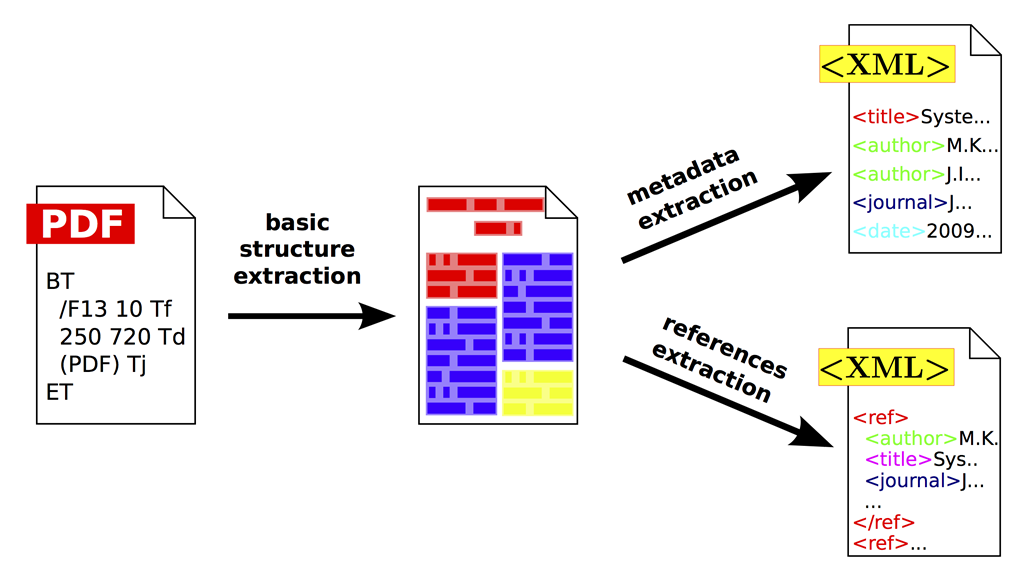
\includegraphics[width=0.7\linewidth]{./assets/cermine}
\end{figure}

Com o mapeamento definido ele identifica regiões de acordo com seu conteúdo, as quais ele chama de \textit{zones}. Esta regiões são determinadas a fim de extrair as informações relevantes para cada uma, de maneira a separar, por exemplo, a área destina aos metadados do arquivo. O CERMINE divide estas \textit{zones} da seguinte maneira:

\begin{itemize}
\item \textbf{Metadata:} É a região mais ao alto do documento, onde obtém os metadados, que seriam o resumo, \textit{bib\_info}, tipo, título, afiliação, autores, datas, editores e palavras-chaves.
\item \textbf{References:} Região responsável por identificas detalhes de referências que foram utilizadas no artigo, como título e autores, por exemplo
\item \textbf{Body:} O texto geral do artigo, incluindo equações, imagens e tabelas.
\item \textbf{Other:} Outros detalhes menos significantes semanticamente, como número das páginas, dentro outros.
\end{itemize}

A extração das referências abrange também seus próprios metadados. Tanto no texto corrido (\textit{Body}) quanto na lista de referências do artigo o \textit{parser} do CERMINE analisa linha a linha, permitindo uma extração de dados mais eficaz. Das referências são extraídos os seguintes dados: autor, título, nome do journal, volume, \textit{issue}, páginas, \textit{publisher}, localização e o ano.

% TeamBeam

Outros projeto de destaque é o TeamBean \cite{teambeam}, cuja base ideológica possui objetivos bem sociais, de contribuir com o compartilhamento de conhecimento. Basicamente o objetivo do projeto é extrair metadados de artigos científicos, porém focado apenas nestes, de maneira a extrair título, nome do \textit{journal}, resumo e informações sobre os autores, como nome, endereço de email e afiliações.




% Falar de cada trabalho encontrado com base nos eventos

	% Falar um resumo
	% Diferencial do projeto
	% Se está ativo ou não
	

	 

\chapter{Metodologia}

Este trabalho tem como metodologia uma pesquisa de caráter não-experimental e quantitativa, por se tratar de coleta de informações e comparação de resultados de técnicas de extração de metadados em artigos científicos.

Desta maneira, a pesquisa de modo padrão não traz alteração nos ambientes pesquisados, apenas os analisa e os compara com base em padrões estabelecidos como sendo de resultado adequado. Assim, o projeto em si trata muito mais de pré-seleção de documentos e técnicas a serem testadas como também dos resultados já analisados e que são necessários para uma técnica ser considerada produtiva.

% Explicar o passo-a-passo que será utilizado

Primeiramente, são filtradas as técnicas encontradas a fim de analisar realmente as que são necessárias dentro do objetivo da pesquisa, fazendo do projeto o mais conciso possível. Desta forma, diversos elementos serão utilizados a fim de se obter os resultados desejados. Os elementos se relacionam entre si e estão identificados na figura \ref{fig:metodology}. 

% Colocar diagrama demonstrando a relação entre todos os objetos, como artigos, técnicas, o processamento, a planilha de resultados e as conclusões

\begin{figure}
\centering
\caption{Processo de Metodologia}
\label{fig:metodology}
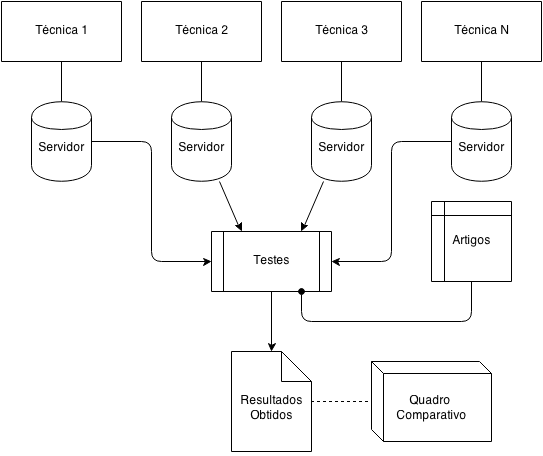
\includegraphics[width=0.7\linewidth]{./assets/metodology}
\end{figure}


\section{Seleção das Técnicas}

As técnicas que foram selecionadas dentro do capítulo de Revisão de Literatura compreendem um universo atuante e de caráter livre, independente da linguagem de programação que foi utilizada, exceto pelos detalhes explicados nas limitações do trabalho.

Assim sendo, todas as técnicas catalogadas e definidas como sendo importantes serão testadas de maneira completa e independente, ou seja, sem interferência de nenhuma outra técnica em seus resultados finais.

% Colocar uma tabela com as técnicas que serão comparadas

\section{Seleção de Artigos}

Visando provar a eficiência destas técnicas, desejamos ter informações de saída consideradas corretas para que seus resultados possam ser comparados e verificados com exatidão. Assim, foi selecionada uma série de artigos científicos das mais diversas áreas de pesquisa, de diversos eventos distintos, com padrões visuais totalmente diferentes e que são possível de ser analisados e coletados.

% Áreas dos Artigos e Eventos

Desde modo a lista destes artigos compreende um total de 100 artigos variados, com seus metadados já extraídos manualmente e todos catalogados a fim de terem o resultado da aplicação das técnicas comparado com os resultados desejados. As áreas do conhecimento, seus respectivos eventos e o número de artigos de cada um estão identificados na Tabela \ref{tab:papers-list}.

Os artigos foram selecionados tomando como base a principal forma de análise das técnicas selecionadas para testes: o layout, ou seja, a disposição dos elementos nos artigos científicos. Esta seleção foi feite com base a abranger um maior número de representações, com disposições diferentes, tipografias diferentes e inclusive ordem diferentes nas exibições. Desta forma as técnicas poderão ser confrontadas e os resultados comparados com os resultados esperados.

% Artigos em Inglês, somente

Todos os artigos selecionados foram escritos na língua inglesa. Esta decisão foi tomada em virtude de além de ser a língua inglesa universal para disseminação de conhecimento, ela é a mais utilizada no meio acadêmico, de maneira a ter um universo muito maior de artigos escrito em inglês do que outras línguas.

Além disso a abrangência de outros idiomas entraria em um aspecto que não é objetivo deste trabalho abordar, visto a diversificação de culturas e símbolos, fazendo com que línguas orientais, como o mandarim ou japonês, tenham análises diferenciadas em função de suas diferenças na forma de representação.

\begin{table}
    \caption{Seleção de artigos científicos para testes (ainda em desenvolvimento)}
    \begin{center}
        \begin{tabular}{l|l|l}
            Área de Conhecimento & Evento ou Conferência & Total de Artigos \\ 
            \hline
            Arquitetura e Urbanismo & Nome do Evento I & 4 \\ 
			Arquitetura e Urbanismo & Nome do Evento II & 3 \\ 
			Artes e Música & Nome do Evento I & 3 \\ 
			Artes e Música & Nome do Evento II & 2 \\ 
            Ciência da Computação & Nome do Evento I & 2 \\
			Ciência da Computação & Nome do Evento II & 4 \\
            Ciência da Informação & ENANCIB 2013 & 4 \\
            Ciência da Informação & Nome do Evento & 3 \\
            Ciências Biológicas & Nome do Evento I & 4 \\
            Direito & Nome do Evento I & 3 \\
            Engenharia Civil & Nome do Evento I & 2 \\
            Medicina & Nome do Evento I & 2 \\ 
            Medicina & Nome do Evento II & 3 \\ 
            Psicologia & Nome do Evento I & 3 \\
            ... & ... & ... \\
            \hline
             & & \textbf{100}
        \end{tabular}
    \end{center}
    \label{tab:papers-list}
\end{table}

\section{Infraestrutura Computacional}

Para que os testes sejam feitos de maneira adequada e independente, sem interferência de outras técnicas nos resultados, serão utilizados N servidores, sendo N o número total de técnicas a serem avaliadas.

Deste modo, para cada técnica avaliada será configurado um servidor com as linguagens de programação necessárias e todos os pré-requisitos que a técnica necessita para funcionar. Estes servidores serão definidos utilizando infraestrutura em \textbf{nuvem} (\textit{Cloud Computing}), o que traz benefícios não somente de performance mas de flexibilidade quanto das tecnologias necessárias para o funcionamento de cada técnica.

 % Falar sobre qual provedor de VPS iremos utilizar
 
Todos os servidores criados para os testes devem necessariamente rodar alguma versão do Linux e serão hospedados nos \textit{data centers} da \textbf{Digital Ocean}\footnote{Acesse o site em \url{http://digitalocean.com}}, empresa de infraestrutura tecnológica de conhecimento mundial e referência em \textit{Cloud Computing} no mercado computacional.

\subsection{Testes In Loco}

% Falar de técnicas que já possuem algum site para testes, demonstrando a ferramente funcionando

Algumas técnicas de extração de metadados disponibilizam acesso online a uma ferramenta gratuita para testes. Deste modo, para estes casos específicos não será necessária a criação de servidores e instalação dos pacotes, visto que o ambiente de testes poderá ser feito dentro da ferramente fornecida pelas desenvolvedoras das técnicas.

% Vantagem de ser feito o teste online

Este fato garante uma maior precisão nos resultados, inclusive pelo fato de o ambiente de testes estar 100\% funcionando e ter sido disponibilizado pela mesma equipe de desenvolvedores do projeto, garantindo a eficácia nos resultados que essa técnicas fornece.

\section{Quadro Comparativo}

Visando uma comparação dos resultados eficaz todos os resultados serão inseridos em um documento formato planilha para serem comparados manualmente e as conclusões então obtidas. Para tal esta planilha de resultados a chamaremos de "Quadro Comparativo" e será exclusiva para comparação dos resultados das técnicas analisadas.

% Formato online para consulta futura

Com o objetivo de facilitar o acesso às informações este documento é disponibilizado como anexo deste projeto e ainda tem seu acesso liberado em formato online. Desta forma qualquer pessoa poderá ter acesso aos resultados obtidos pelos testes e comparar elas mesmas os dados contidos na planilha.

\section{Metadados, Pesos e Resultados}

% Importância de se ter pesos em função dos metadados

A extração de metadados de artigos científicos engloba um processo onde os resultados obtidos, mais especificamente os metadados propriamente ditos, possuem características diferenciadas que podem influenciar em uma busca por artigos, feita por um pesquisador.

Desde modo atribuímos pesos para cada um dos metadados analisados, de maneira a identificar os mais importantes e que podem contribuir com um número maior de resultados de busca. 

% Quais metadados são mais importantes para uma pesquisa de artigos

Alguns metadados são mais importantes que outros no que diz respeito à funcionalidade de pesquisa. Geralmente quando vamos buscar artigos, seja na Internet, ou em algum outro local, geralmente buscamos primeiro pelo título do artigo (quando procuramos por um artigo em específico) ou então pelo nome do autor (quanto procuramos artigos de um determinado autor).

Além disso, utilizamos também o título, juntamente com o resumo, para buscar de palavras chaves ou palavras que podem ser relevantes na pesquisa pelos documentos. Assim sendo alguns metadados devem ser mais considerados no resultado destas extrações, por serem mais importantes no ponto de vista da busca.

Assim sendo apresentamos a tabela \ref{tab:pesos}, que demonstra como cada metadado teve sua importância interpretada e qual o peso que lhe foi atribuído, sendo utilizado o inteiro 1 para o peso mais baixo e o 5 para peso mais alto, sendo consequentemente o mais importantes.

% Tabela de metadados e pesos

\begin{table}
    \caption{Os metadados e seus pesos atribuídos}
    \begin{center}
    	\begin{tabular}{|p{3cm}|p{8cm}|C{1cm}|}
			\hline \textbf{Metadado} & \textbf{Relevância} & \textbf{Peso} \\ 
			\hline Título & Um dos termos mais buscados quando se pesquisa um artigo & 5 \\
	    	\hline Autor(es) & O segundo termo mais pesquisado & 4 \\
	    	\hline E-mail(s) & Pouco relevante no quesito pesquisa de artigos & 1 \\
	    	\hline Resumo & Importante por conter palavras chaves e o resumo propriamente dito & 3 \\
	    	\hline Referências & Muito importante e necessário, pois será utilizada na referência inversa de autores & 5 \\
	    	\hline 
    	\end{tabular} 
    \end{center}
  	\label{tab:pesos}
\end{table}

% Falar sobre a porcentagem de acertos em cada metadado, por exemplo, se o resultado extraiu 90\% do resultado (não a totalidade), deve ser considerado um valor para este resultado, não somente sim ou não.

Outro detalhe importante é a precisão de cada resultado para cada metadado analisado. Em alguns casos o título, por exemplo, não é extraído em 100\% mas alguma variação dele. 

Deste modo consideramos 3 (três) resultados possíveis para um resultado analisado:

\begin{enumerate}
\item \textbf{Preciso:} Quando um resultado atinge acima de 95\% de precisão, ou seja, o campo foi extraído em 95\% ou mais de sua totalidade.
\item \textbf{Satisfatório:} Quando um resultado atinge entre 90 e 94\%, o que pode ser considerado satisfatório e a maioria do conteúdo consegue ser analisada sem maiores problemas.
\item \textbf{Inaceitável:} Quando o resultado atinge abaixo de 90\%, ou seja, entre 0\% e 89\%. Este resultado no âmbito do presente projeto é considerado inaceitável.
\end{enumerate}

Assim, temos o valor de cada resultado possível, que será também utilizado no processo de análise, conforme consta na tabela \ref{tab:precisao}.

% Tabela de precisão e os valores

\begin{table}
    \caption{Resultados obtidos em cada metadado e sua precisão}
    \begin{center}
    	\begin{tabular}{|C{3cm}|C{3cm}|}
			\hline \textbf{Resultado} & \textbf{Precisão} \\ 
			\hline Preciso & 1\\
	    	\hline Satisfatório & 0.60 \\
	    	\hline Inaceitável & 0 \\
	    	\hline 
    	\end{tabular} 
    \end{center}
  	\label{tab:precisao}
\end{table}

\subsection{Índice de Confiabilidade}

% Fórmula final para a nota final de cada técnica

Considerando que cada metadado possui um peso diferente necessitamos calcular o índice de acertos a ser utilizado em cada resultado coletado para cada técnica aplicada. Assim sendo chegamos em uma fórmula matemática à qual chamamos "Índice de Confiabilidade", que calcula o resultado obtido através dos pesos que foram atribuídos.

Este índice utiliza os pesos anteriormente definidos e a precisão dos resultados obtida, de maneira a permitir chegar em um único resultado para cada técnica aplicada.

\begin{center}
	$ Fórmula a ser definida ainda $
\end{center}


\chapter{Testes}

\section{Ambiente de Testes}

\subsection{Servidores de Teste}

\chapter{Resultados}

\chapter{Conclusão}

\section{Trabalhos Futuros}

\section{Considerações Finais}


% ---

% ----------------------------------------------------------
% ELEMENTOS PÓS-TEXTUAIS
% ----------------------------------------------------------
\postextual
% ----------------------------------------------------------

% ----------------------------------------------------------
% Referências bibliográficas
% ----------------------------------------------------------
\bibliography{references}

% ----------------------------------------------------------
% Glossário
% ----------------------------------------------------------
%
% Consulte o manual da classe abntex2 para orientações sobre o glossário.
%
%\glossary

% ----------------------------------------------------------
% Apêndices
% ----------------------------------------------------------

% ---
% Inicia os apêndices
% ---
% \begin{apendicesenv}

% % Imprime uma página indicando o início dos apêndices
% \partapendices

% % ----------------------------------------------------------
% \chapter{Quisque libero justo}
% % ----------------------------------------------------------

% \lipsum[50]

% % ----------------------------------------------------------
% \chapter{Nullam elementum urna vel imperdiet sodales elit ipsum pharetra ligula
% ac pretium ante justo a nulla curabitur tristique arcu eu metus}
% % ----------------------------------------------------------
% \lipsum[55-57]

% \end{apendicesenv}
% ---


% ----------------------------------------------------------
% Anexos
% ----------------------------------------------------------

% ---
% Inicia os anexos
% ---
% \begin{anexosenv}

% % Imprime uma página indicando o início dos anexos
% \partanexos

% % ---
% \chapter{Morbi ultrices rutrum lorem.}
% % ---
% \lipsum[30]

% % ---
% \chapter{Cras non urna sed feugiat cum sociis natoque penatibus et magnis dis
% parturient montes nascetur ridiculus mus}
% % ---

% \lipsum[31]

% % ---
% \chapter{Fusce facilisis lacinia dui}
% % ---

% \lipsum[32]

% \end{anexosenv}

%---------------------------------------------------------------------
% INDICE REMISSIVO
%---------------------------------------------------------------------
\phantompart
\printindex
%---------------------------------------------------------------------

\end{document}
